% !TEX root = thesis.tex
\begin{appendices}

\section{Additional graphs}
\label{app:a}

\begin{figure}
\centering
%\begin{subfigure}{0.24\textwidth}
%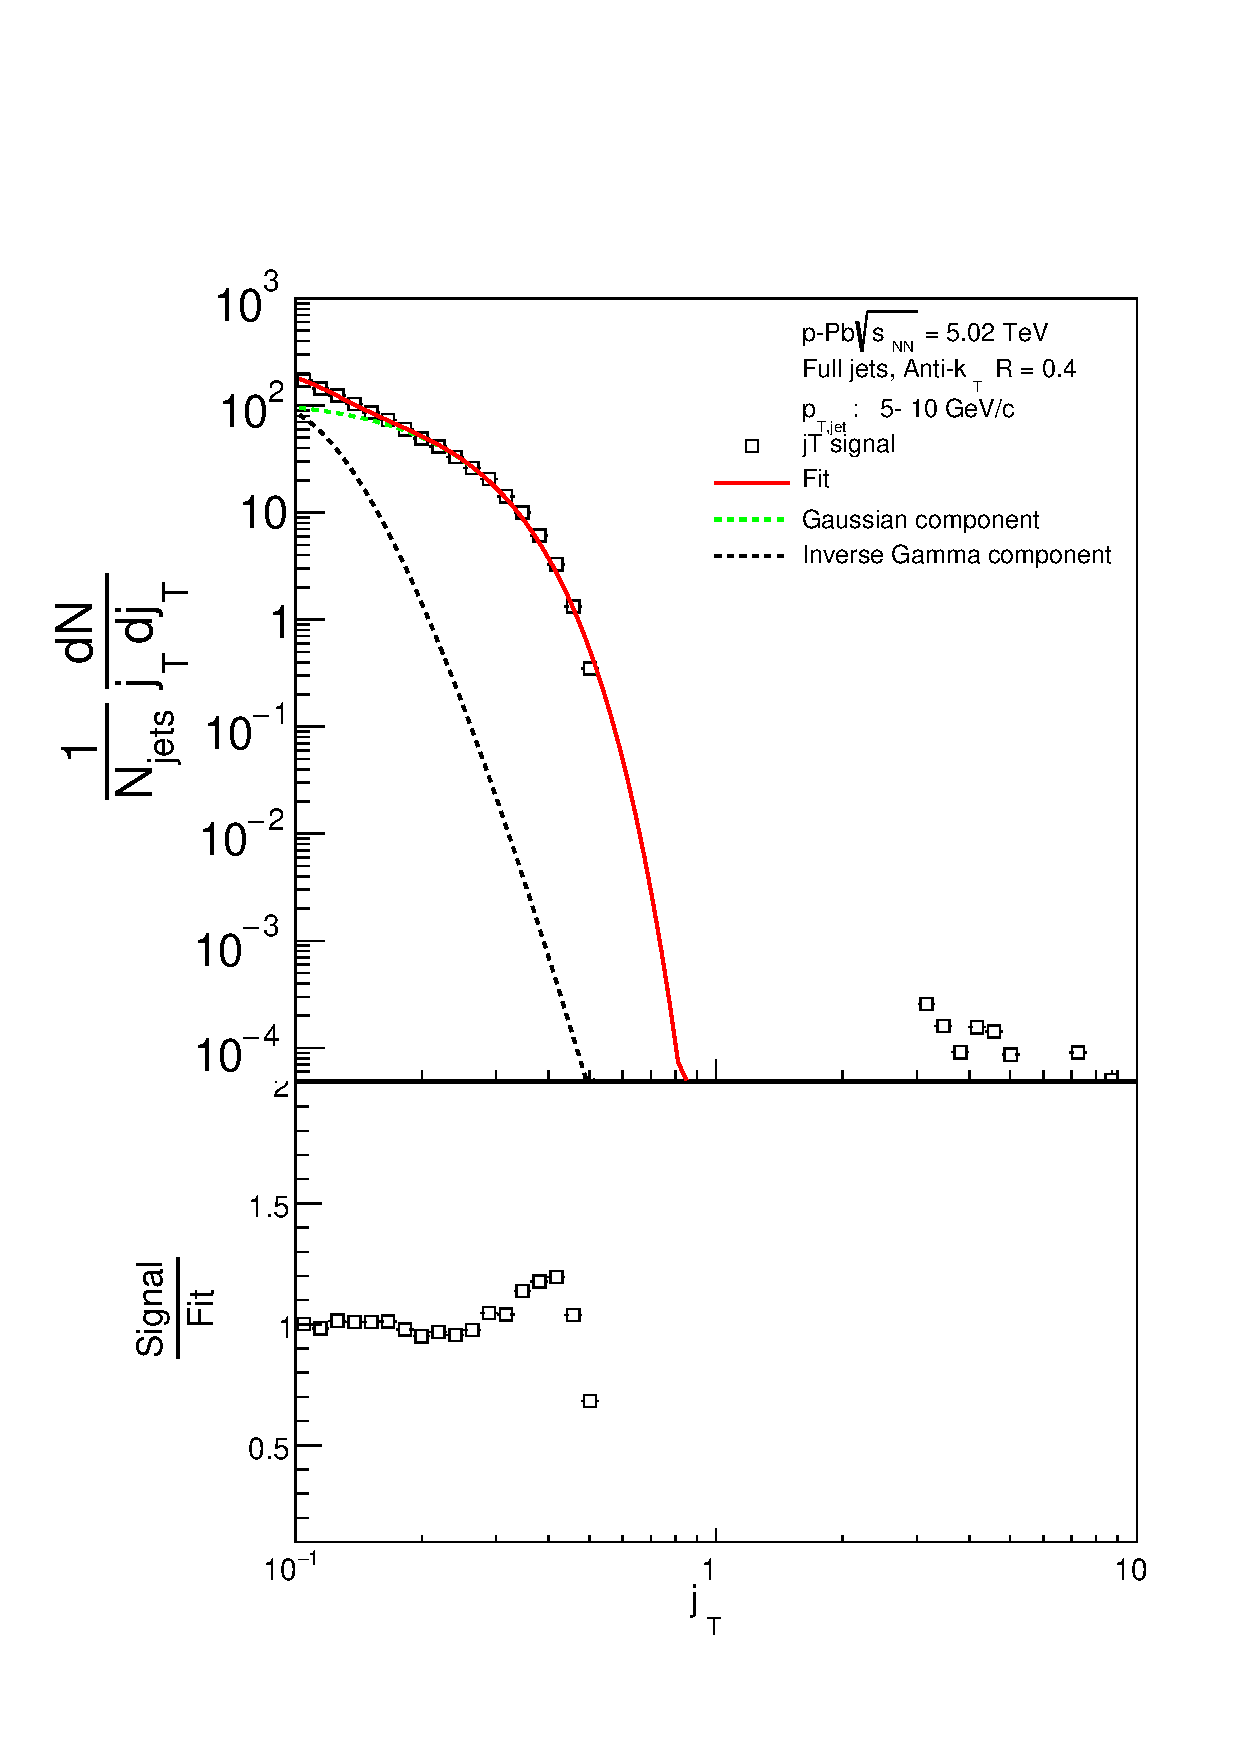
\includegraphics[width=0.95\textwidth]{results/JetConejTSignalFit/JetConejTSignalFitNFin00JetPt00perconeBgBayes}
%\end{subfigure}
%\begin{subfigure}{0.24\textwidth}
%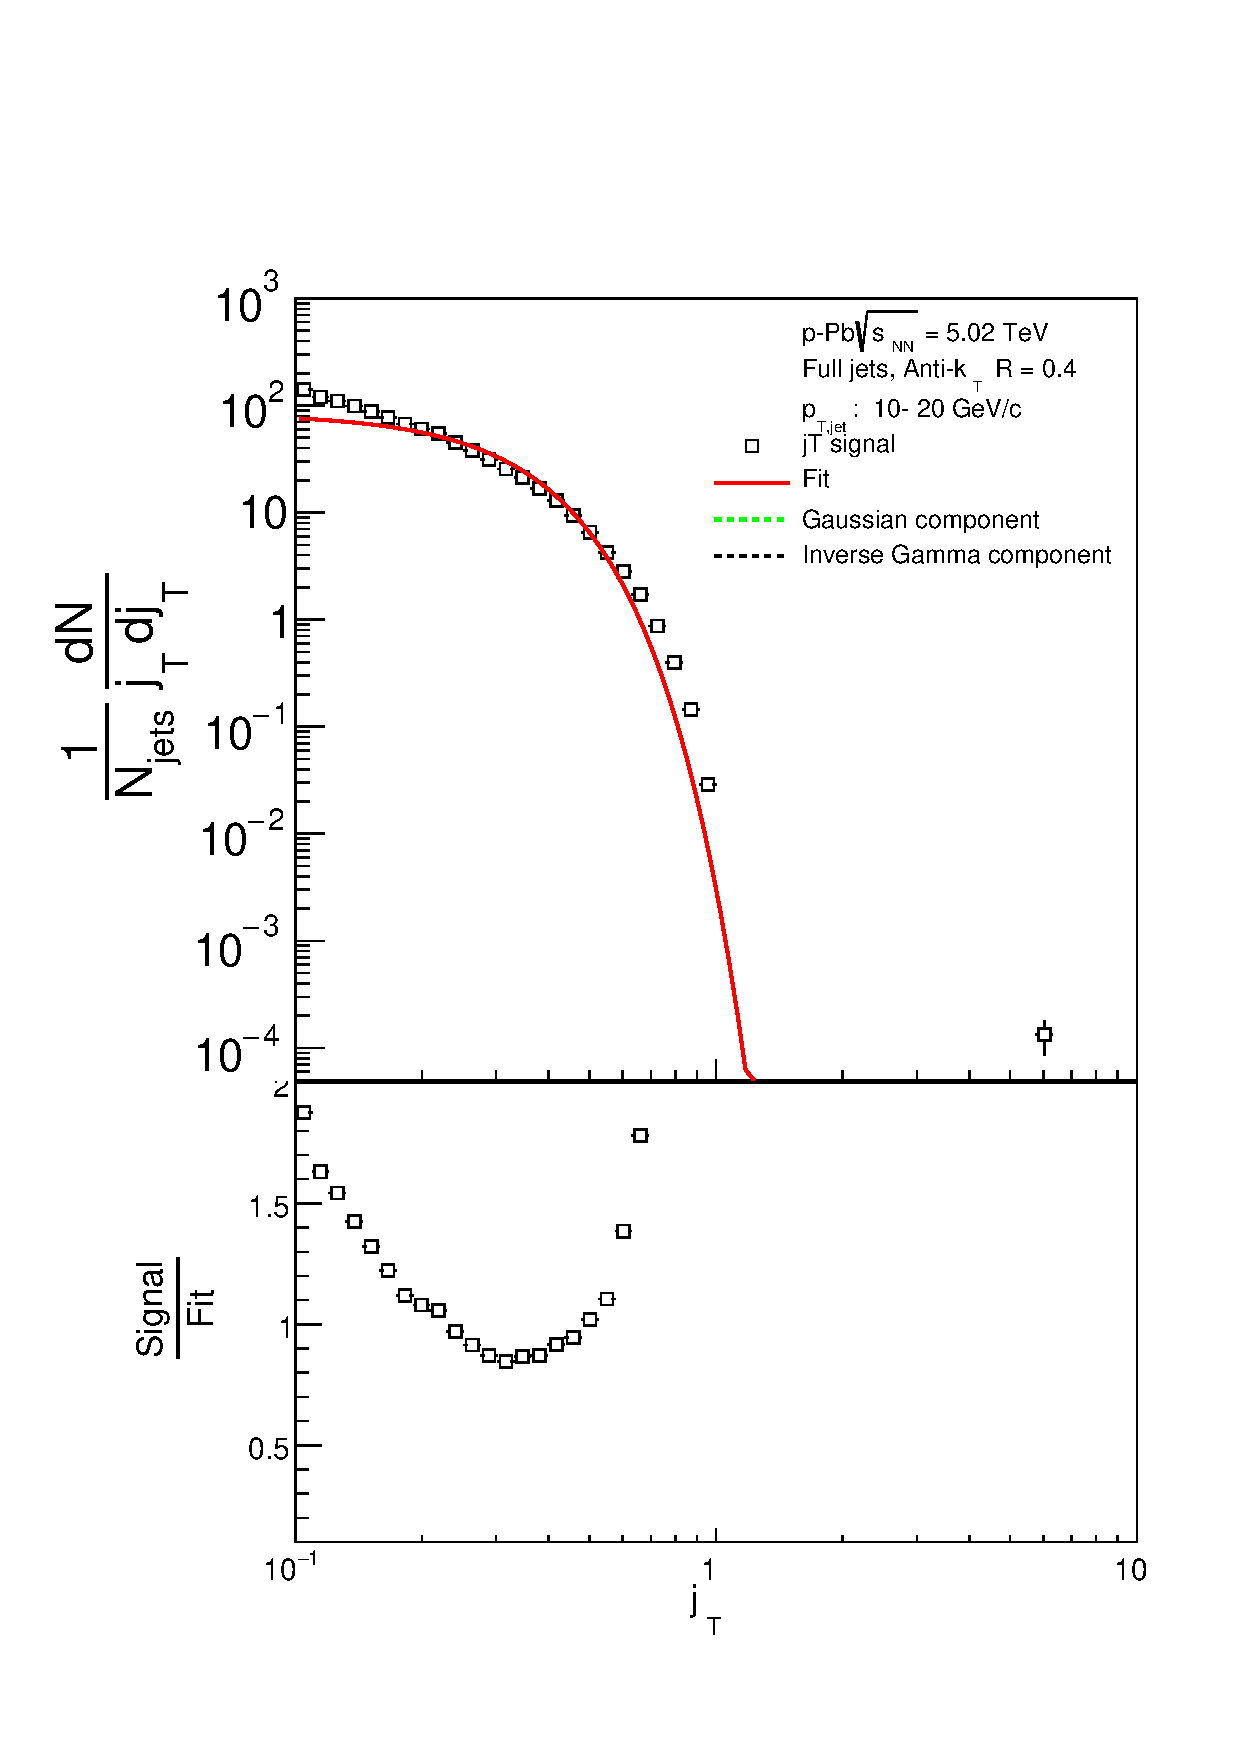
\includegraphics[width=0.95\textwidth]{results/JetConejTSignalFit/JetConejTSignalFitNFin00JetPt01perconeBgBayes}
%\end{subfigure}
%\begin{subfigure}{0.24\textwidth}
%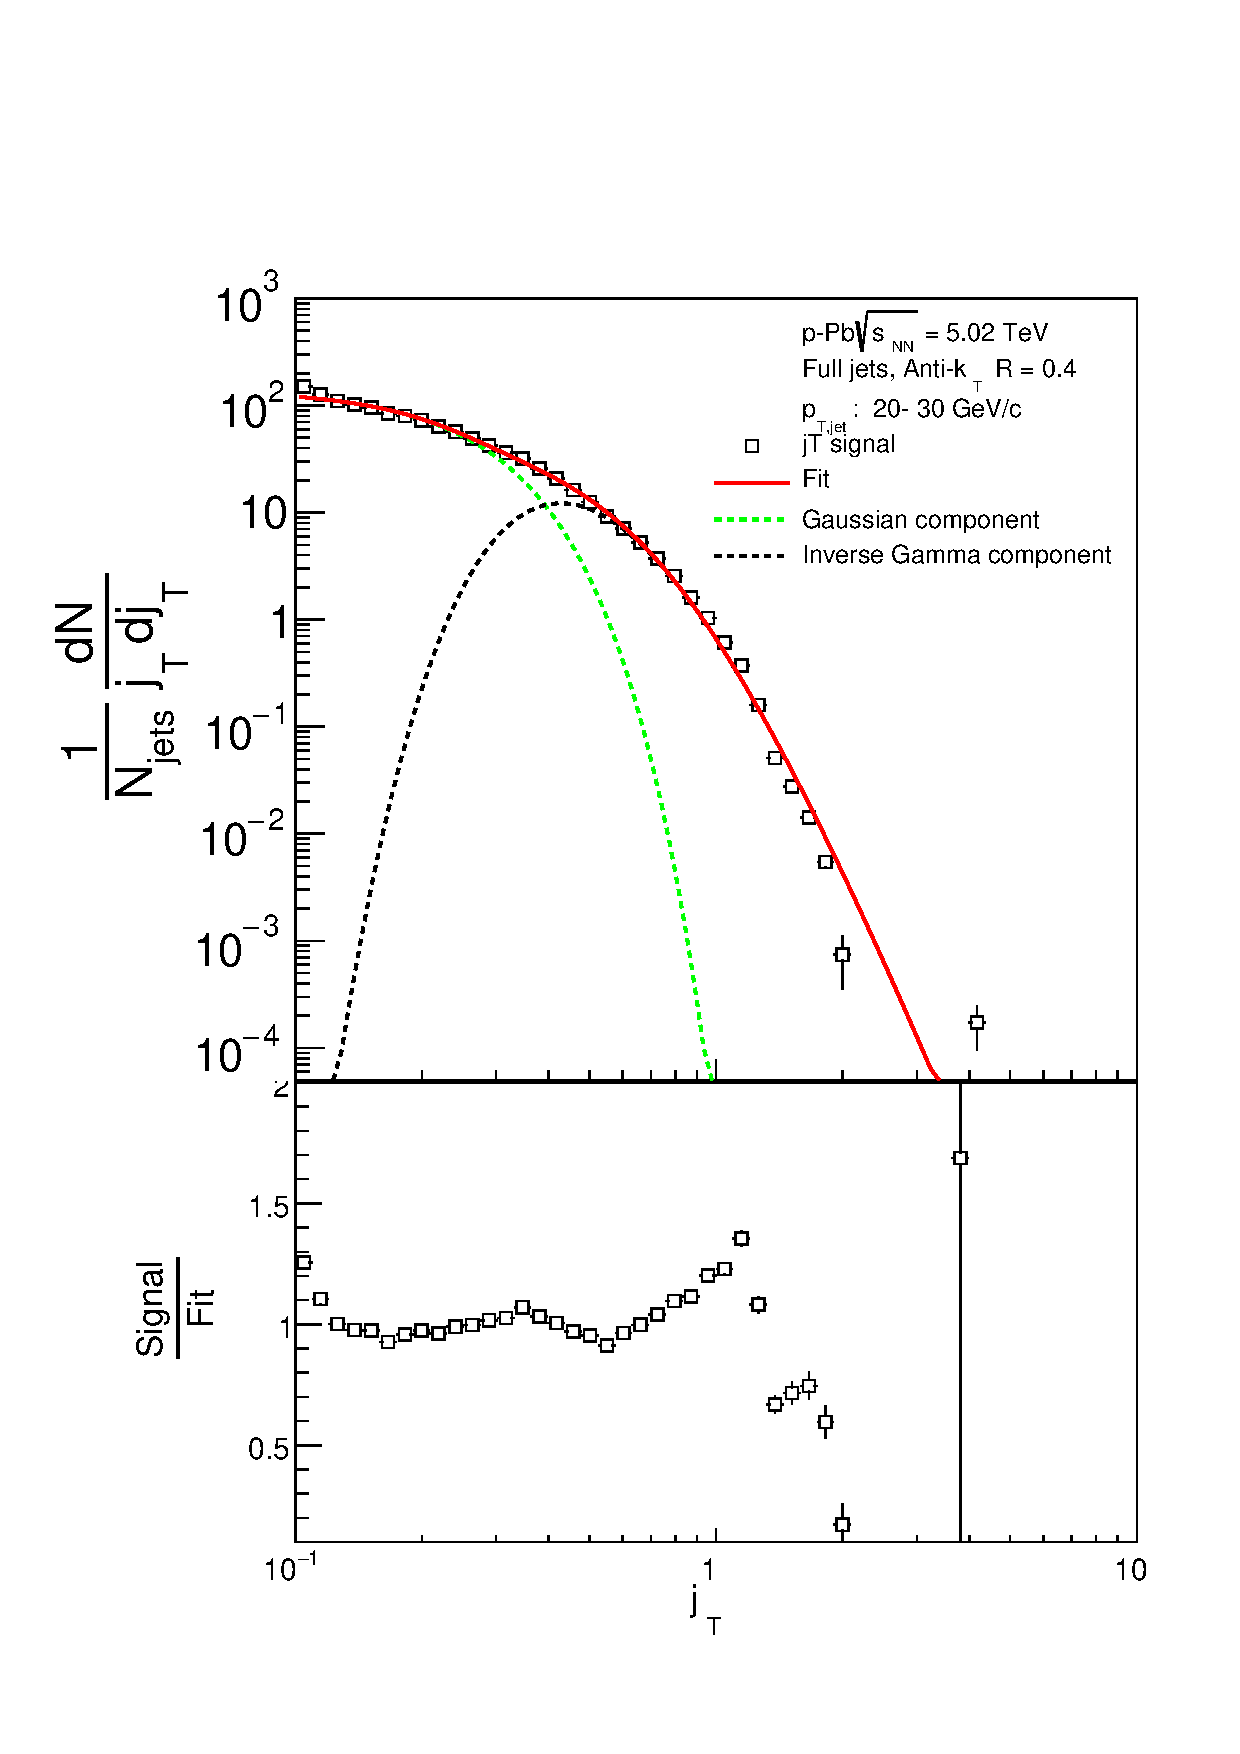
\includegraphics[width=0.95\textwidth]{results/JetConejTSignalFit/JetConejTSignalFitNFin00JetPt02perconeBgBayes}
%\end{subfigure}
\begin{subfigure}{0.24\textwidth}
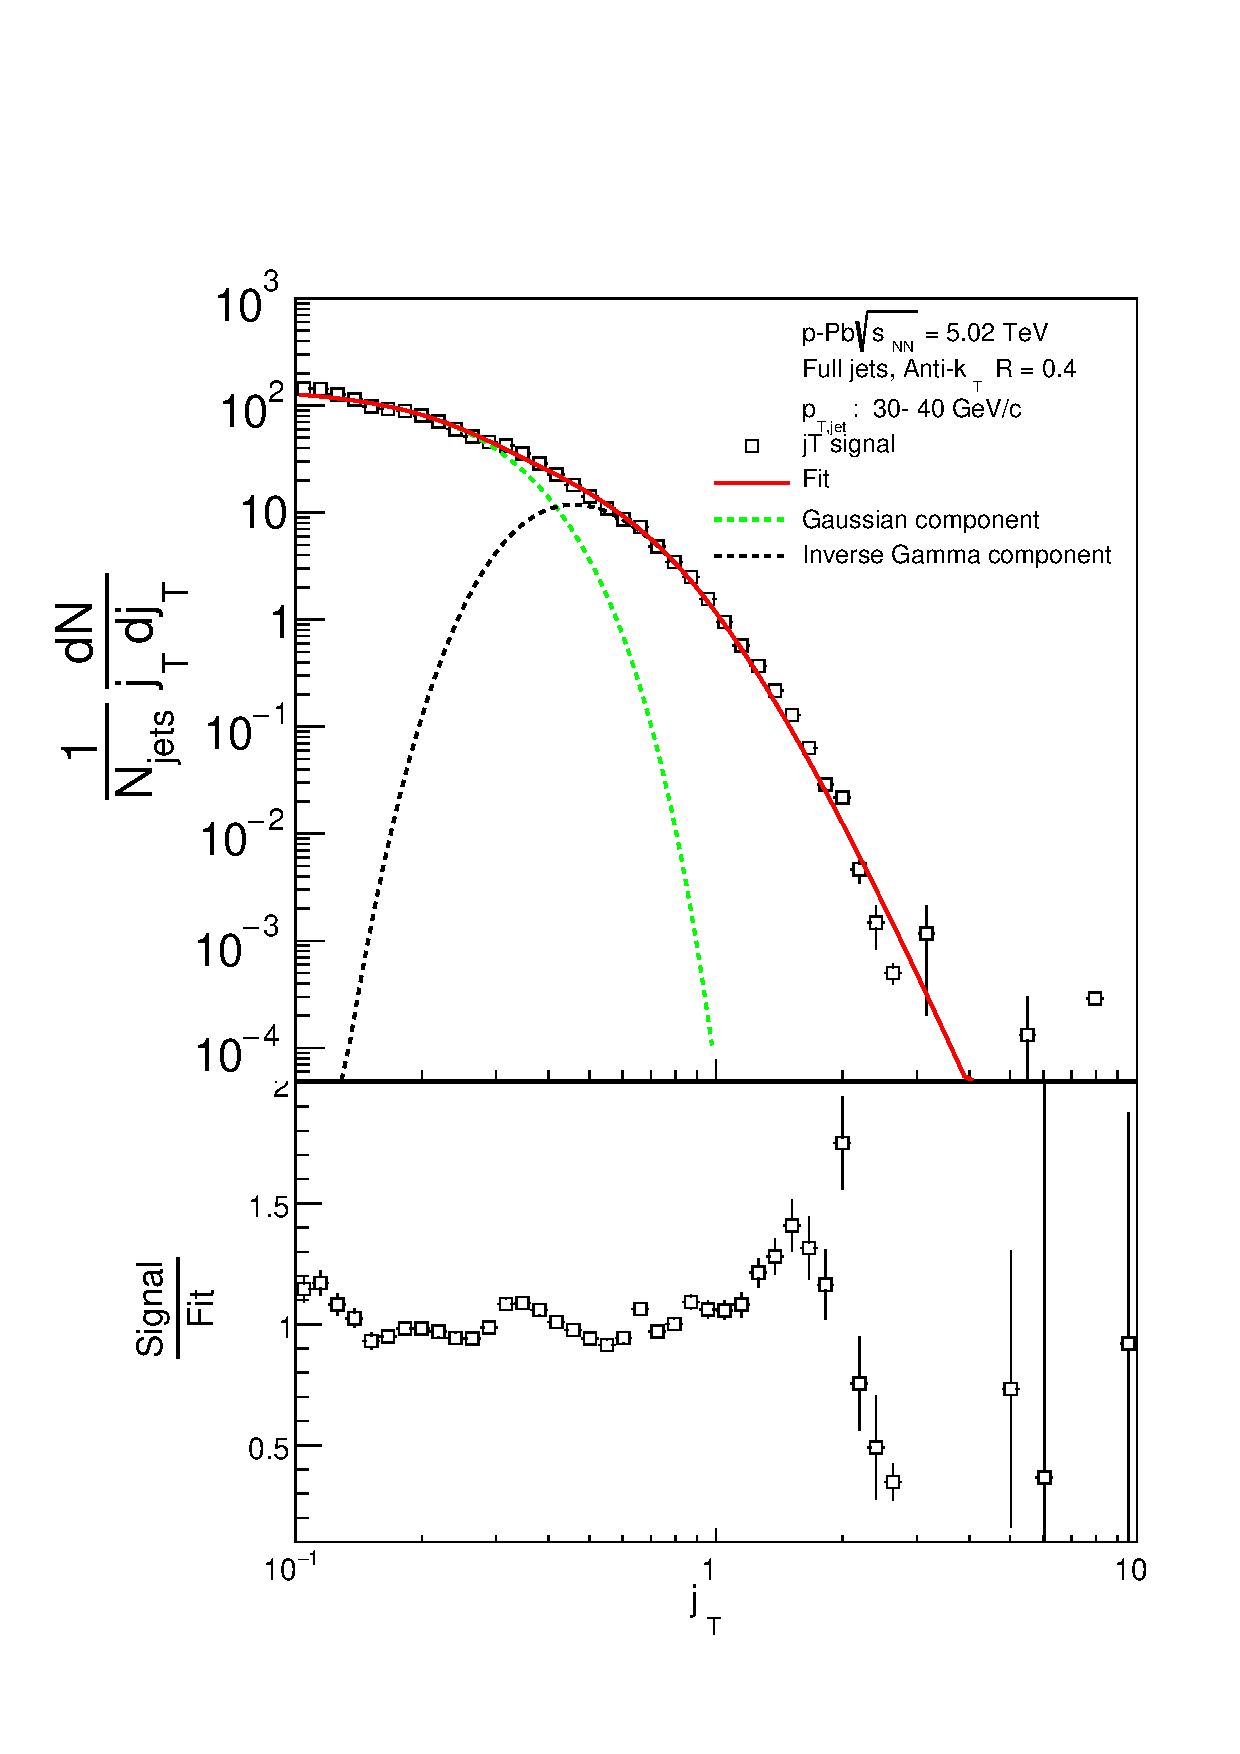
\includegraphics[width=0.95\textwidth]{results/JetConejTSignalFit/JetConejTSignalFitNFin00JetPt03perconeBgBayes}
\end{subfigure}
\begin{subfigure}{0.24\textwidth}
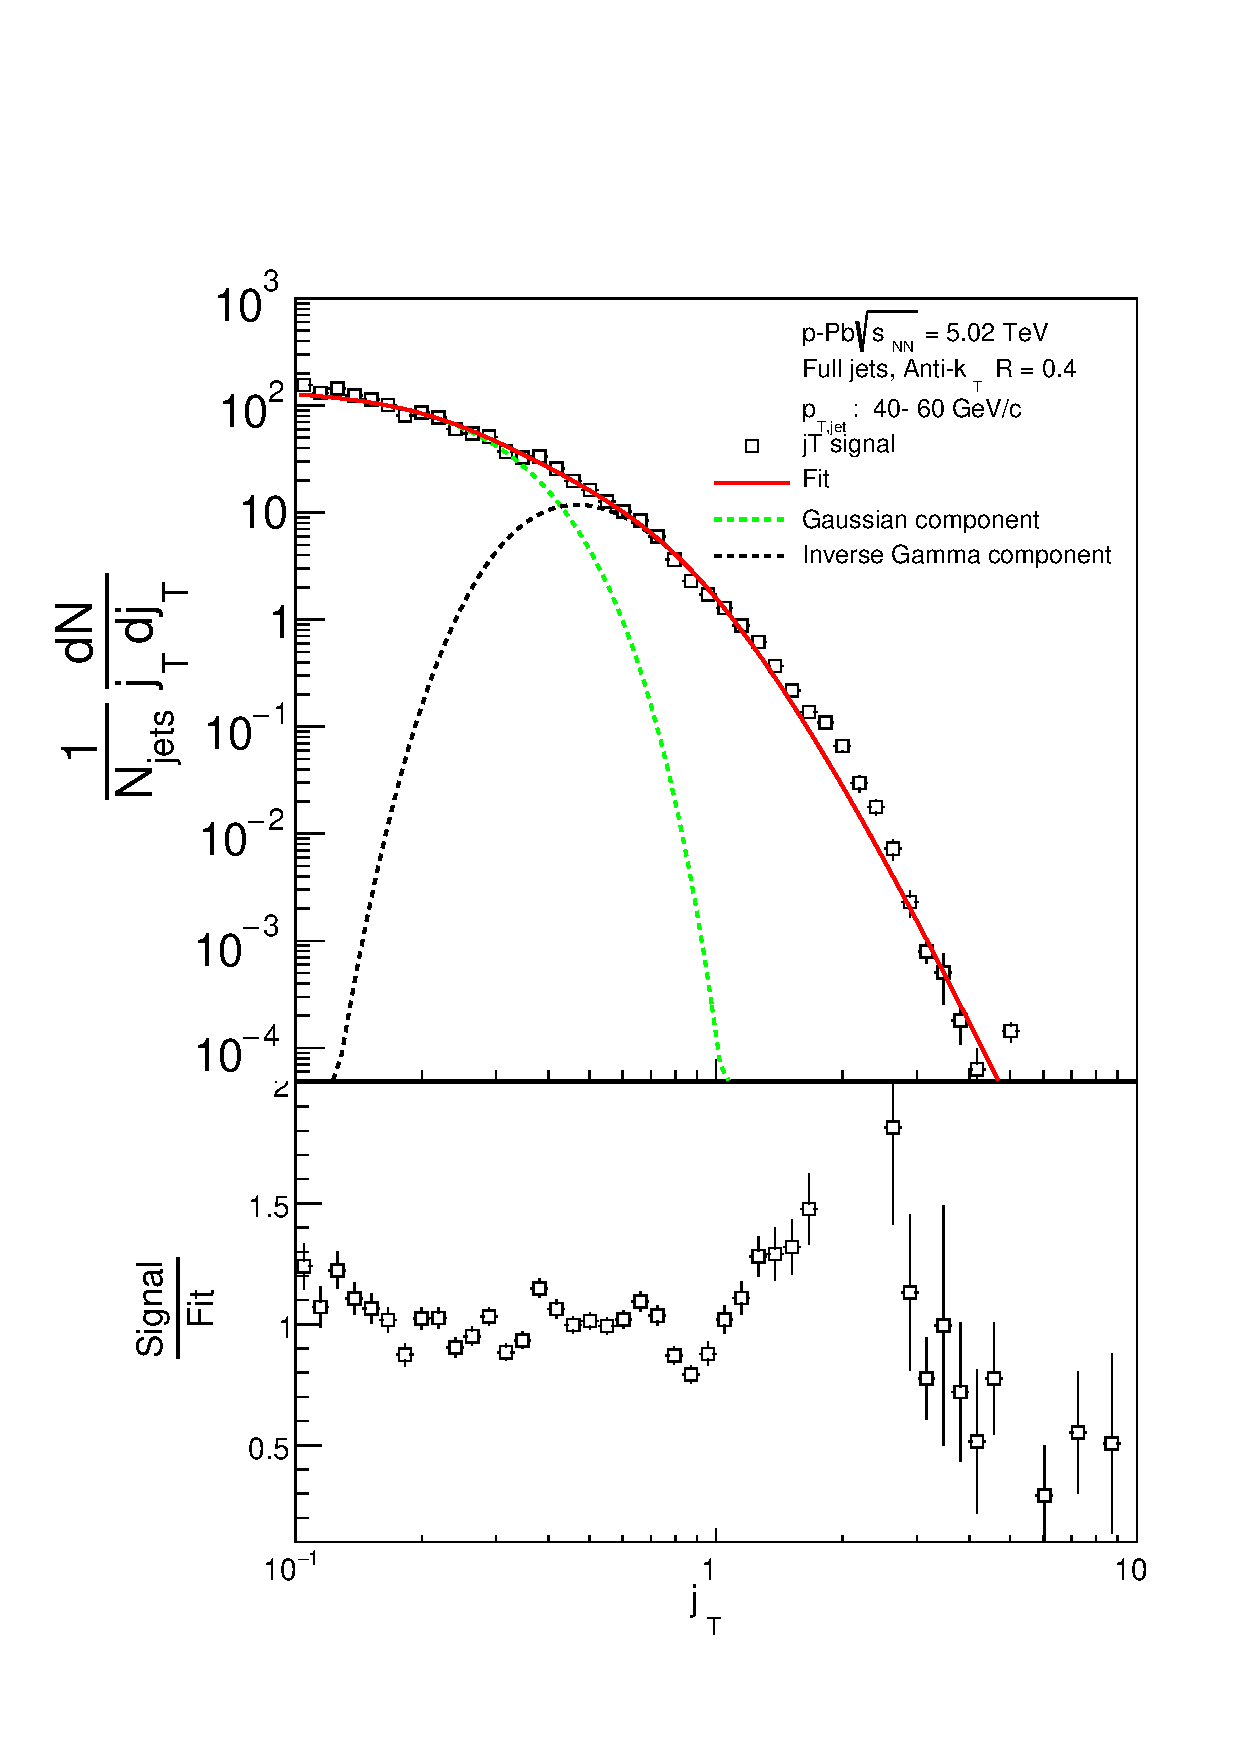
\includegraphics[width=0.95\textwidth]{results/JetConejTSignalFit/JetConejTSignalFitNFin00JetPt04perconeBgBayes}
\end{subfigure}
\begin{subfigure}{0.24\textwidth}
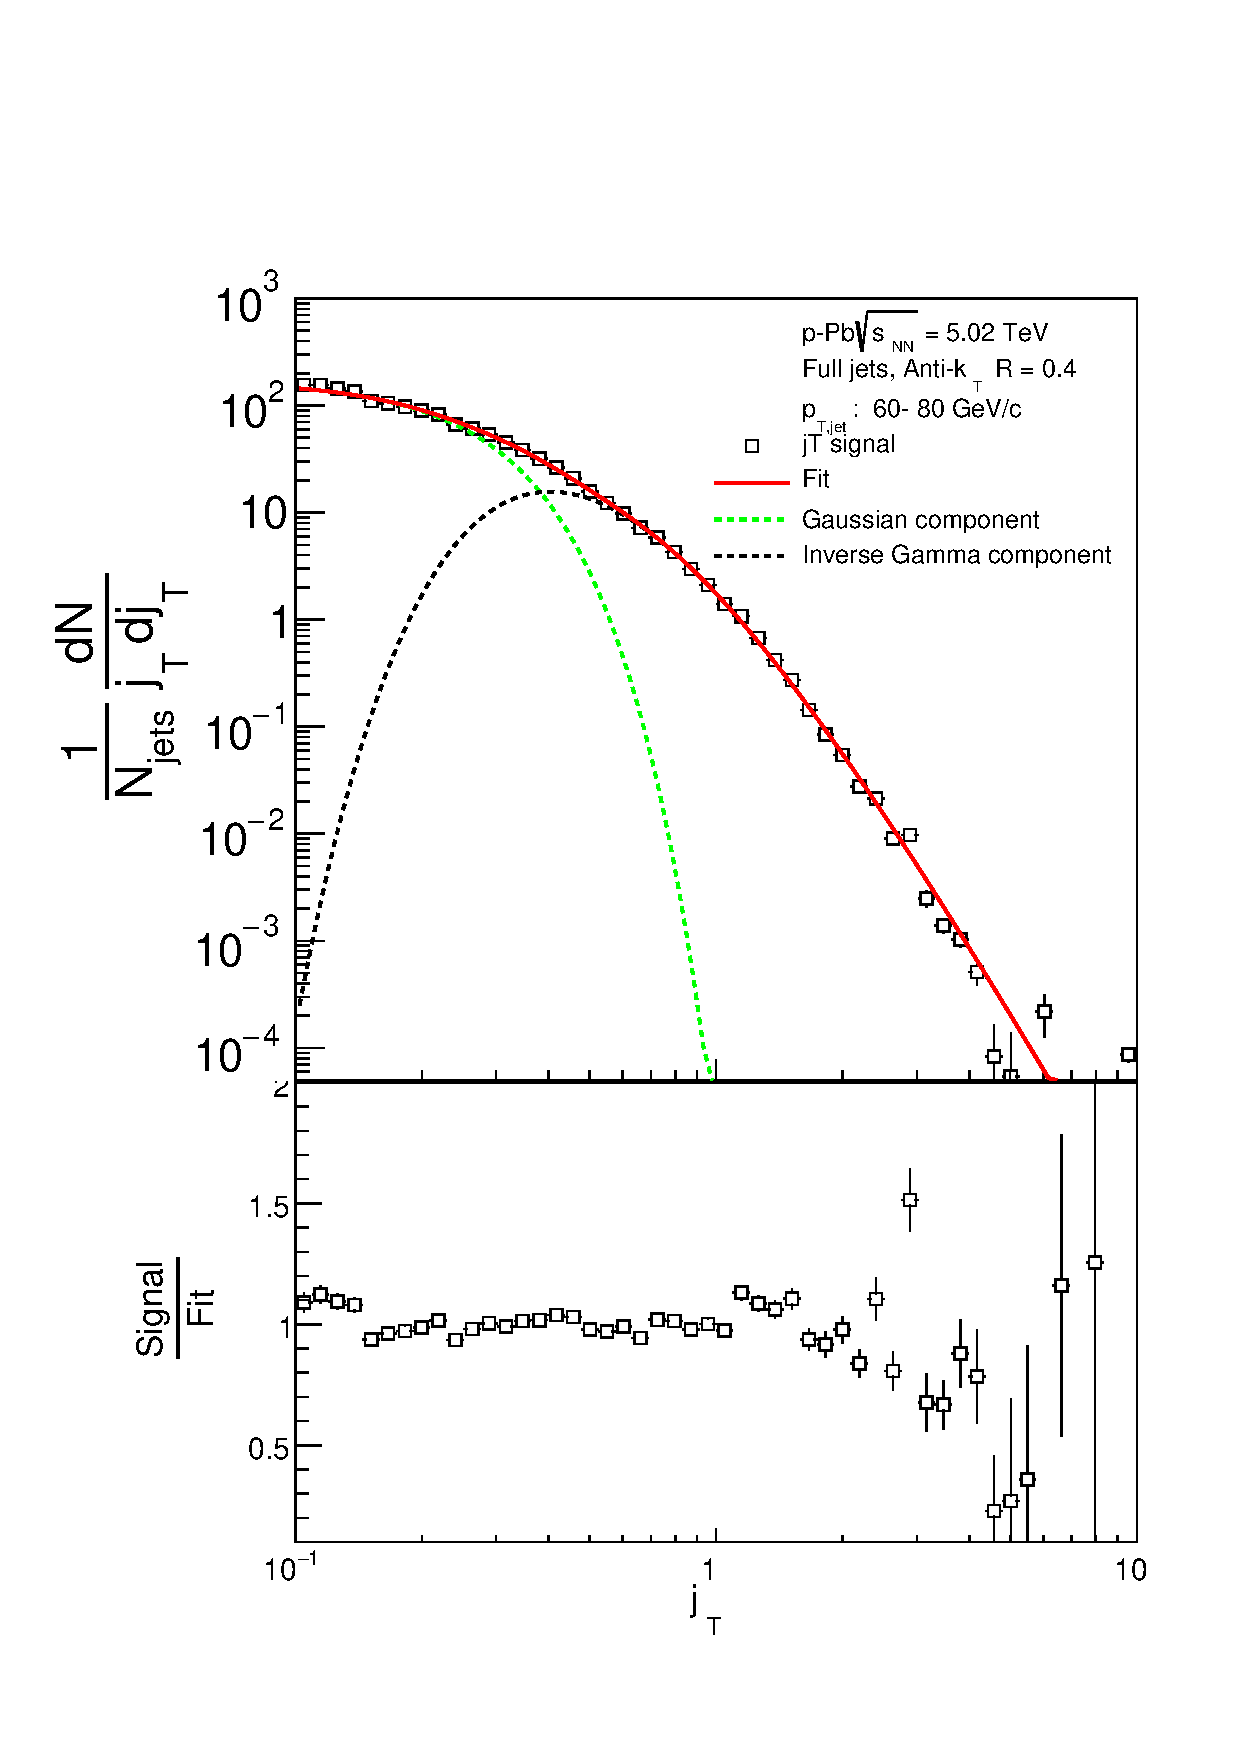
\includegraphics[width=0.95\textwidth]{results/JetConejTSignalFit/JetConejTSignalFitNFin00JetPt05perconeBgBayes}
\end{subfigure}
\begin{subfigure}{0.24\textwidth}
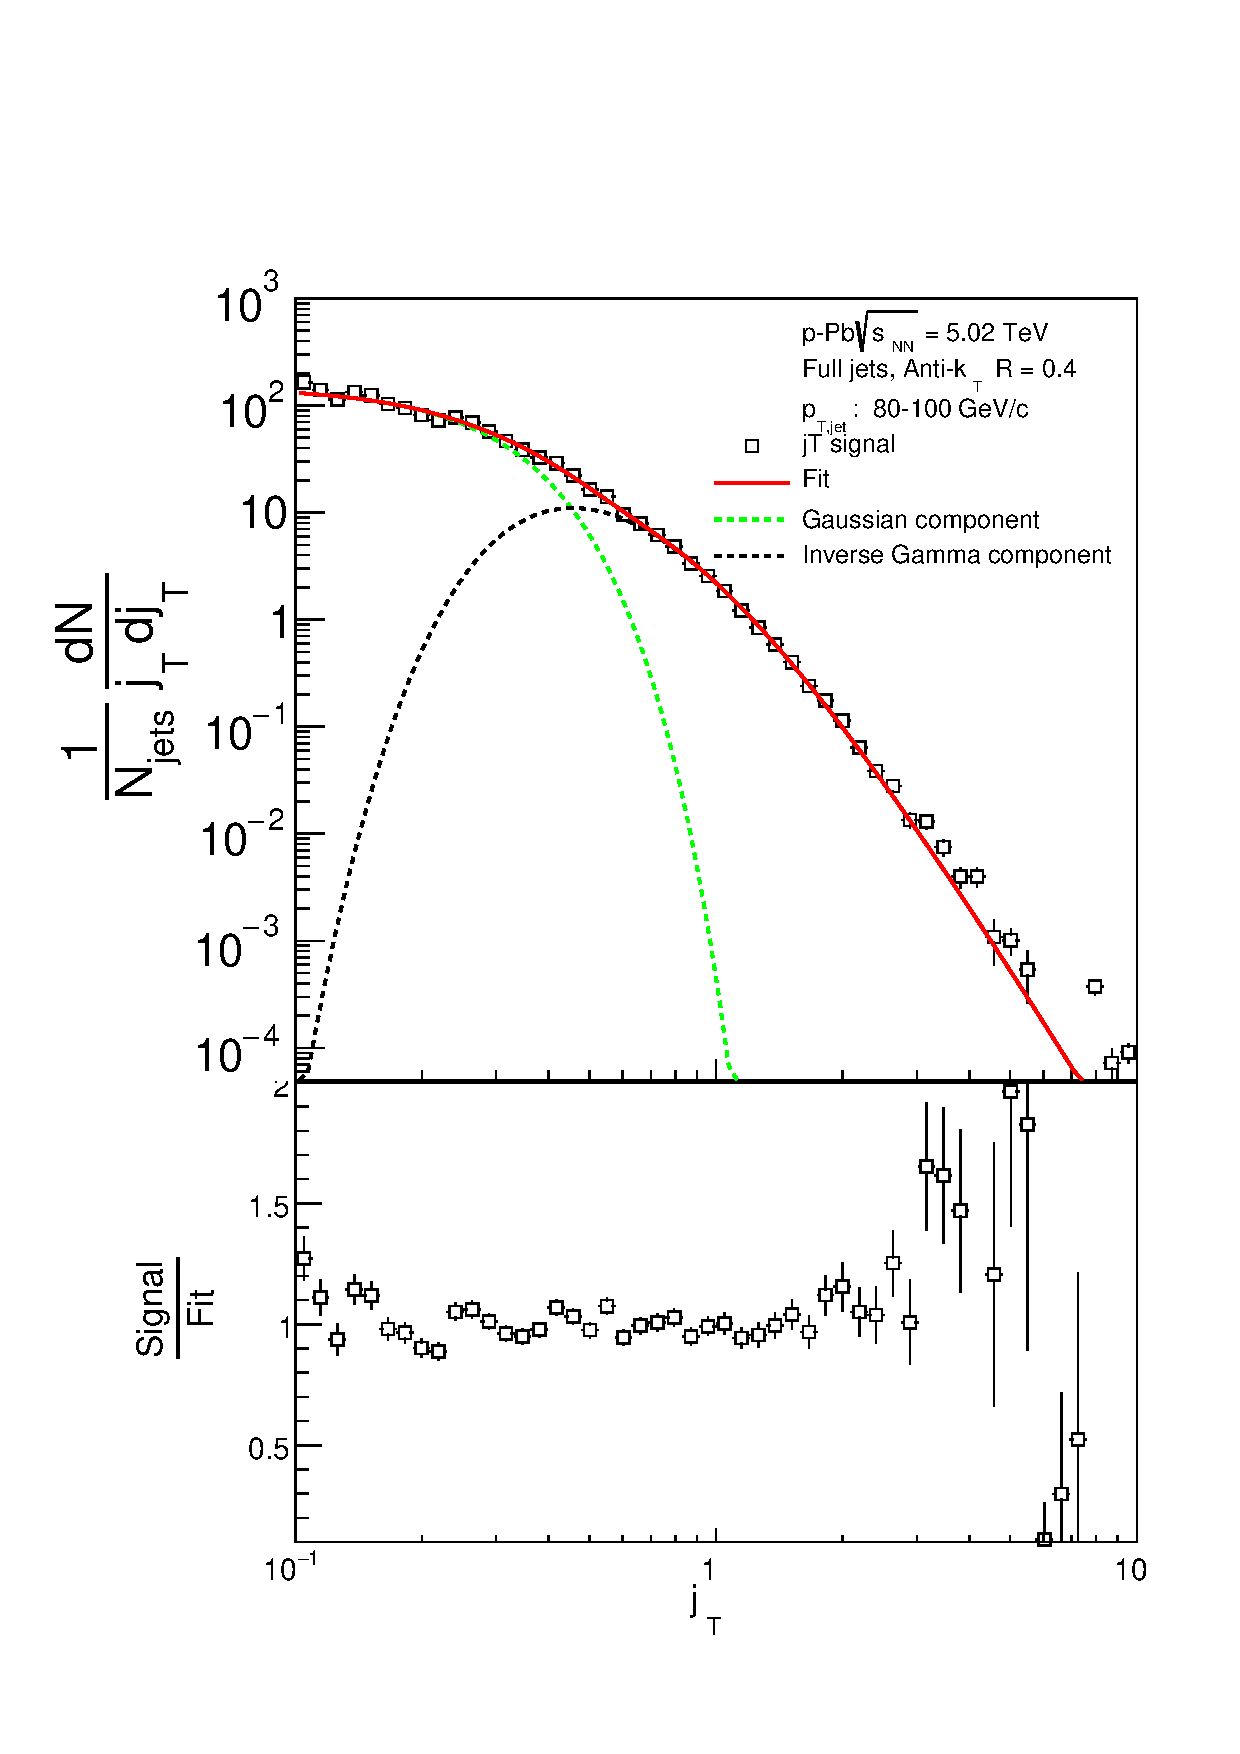
\includegraphics[width=0.95\textwidth]{results/JetConejTSignalFit/JetConejTSignalFitNFin00JetPt06perconeBgBayes}
\end{subfigure}
\begin{subfigure}{0.24\textwidth}
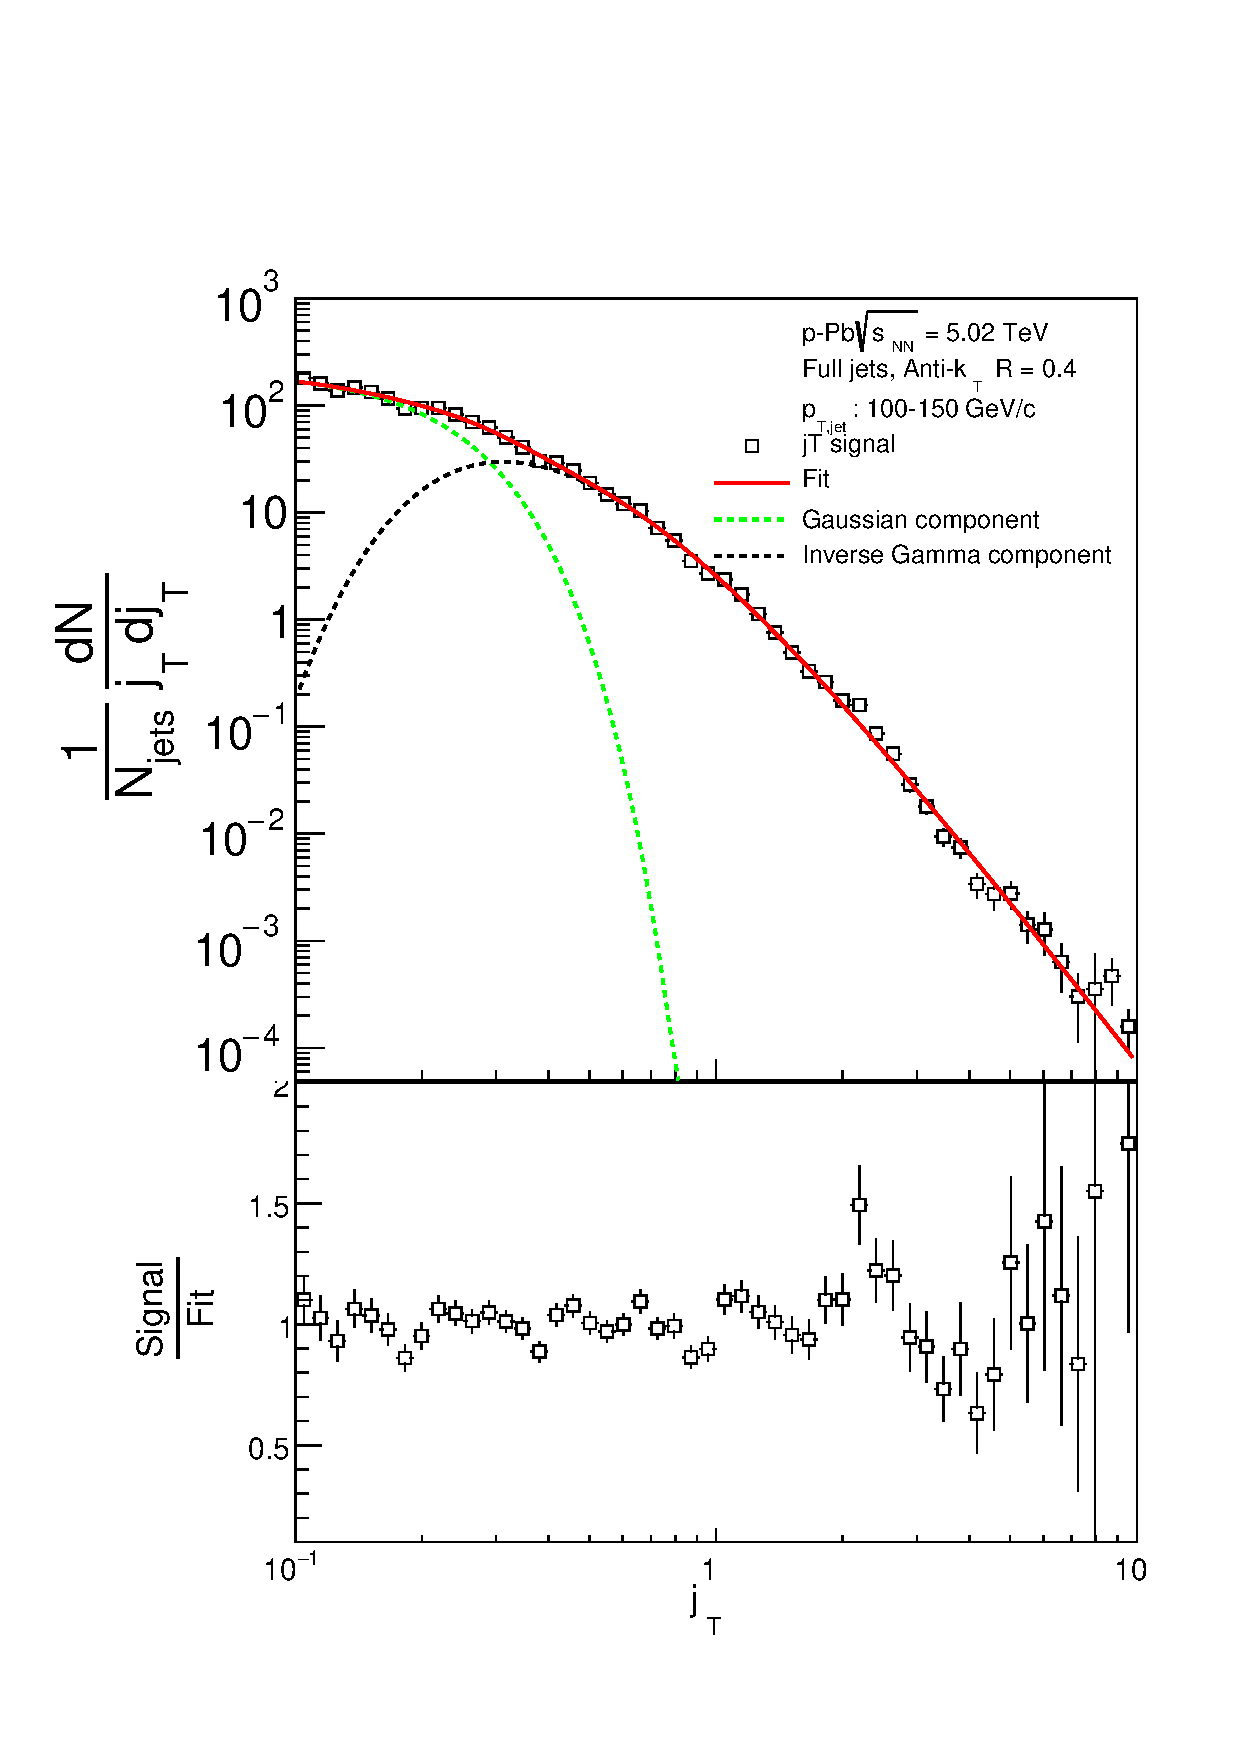
\includegraphics[width=0.95\textwidth]{results/JetConejTSignalFit/JetConejTSignalFitNFin00JetPt07perconeBgBayes}
\end{subfigure}
\caption{$\jt{}$ signal fits in different jet $\pt{}$ bins}
\label{fig:fits}
\end{figure}


\end{appendices}